\documentclass[11pt,letterpaper]{article}
\usepackage[lmargin=1in,rmargin=1in,tmargin=1in,bmargin=1in]{geometry}
\usepackage{homework}

% -------------------
% Content
% -------------------
\begin{document}
\homework{\textit{Caleb McWhorter --- Solutions}}

% Problem 1
\problem{10} Consider the following graph:
	\[
	\graphOne
	\]

\begin{enumerate}[(a)]
\item Is the graph directed or undirected?
\item Give the vertex set and the edge set for the graph.
\item Give the adjacency matrix of the graph.
\item Is the graph simple?
\item Are there any isolated vertices?
\item List all pairs of parallel edges.
\item Compute the degree of the graph.  
\item Are the vertices $v_1$ and $v_6$ connected? What about the vertices $v_1$ and $v_4$? 
\item Does the graph $G \setminus \{ v_6 \}$ have an Eulerian circuit? Find one or explain why none exists.  
\item Does the graph $G \setminus \{ v_6 \}$ have an Hamiltonian circuit? Find one or explain why none exists.  
\end{enumerate} \pspace

\sol
\begin{enumerate}[(a)]
\item This graph is undirected as there is no direction/orientation to the edges. 

\item We have\dots
	\[
	\begin{aligned}
	V(G)&= \{ v_1, v_2, v_3, v_4, v_5, v_6 \} \\[0.3cm]
	E(G)&= \{ e_1, e_2, e_3, e_4, e_5, e_6, e_7, e_8 \} \\
	&= \{ \{v_1, v_3\}, \{v_1, v_2\}, \{v_2, v_3\}, \{v_2, v_3\}, \{v_2, v_4\}, \{v_3, v_4\}, \{v_3, v_5\}, \{v_4, v_5\} \}
	\end{aligned}
	\]

\item The adjacency matrix is $A= (a_{ij})$, where $a_{ij}$ is the number of edges from vertex $i$ to vertex $j$. But then the adjacency matrix is\dots
	\[
	A= 
	\begin{pmatrix}
	0 & 1 & 1 & 0 & 0 & 0 \\
	1 & 0 & 2 & 1 & 0 & 0 \\
	1 & 2 & 0 & 1 & 1 & 0 \\
	0 & 1 & 1 & 0 & 1 & 0 \\
	0 & 0 & 1 & 1 & 0 & 0 \\
	0 & 0 & 0 & 0 & 0 & 0 
	\end{pmatrix}
	\]
Observe that this matrix is symmetric, i.e. $A= A^T$, because the graph is undirected. 

\item A simple graph is a graph without loops or multiple edges. There are multiple edges in this graph because there are two edges between $v_2$ and $v_3$---namely $e_3$ and $e_4$. Therefore, the graph is not simple. 

\item An isolated vertex has no edges coming into or going out of it. Therefore, the only isolated vertex is $v_6$. 

\item Two distinct edges are parallel if they have the same endpoints. The only pair of edges that share the same endpoints are $e_3$ and $e_4$, which share the endpoints $v_2$ and $v_3$. Therefore, $e_3$ and $e_4$ are the only parallel edges. [Not that other edges share \textit{an} endpoint but not \textit{all} endpoints, e.g. $e_1$ and $e_2$ share the endpoint $v_1$ but are not parallel because they do not share the end point $v_2$ or $v_3$.]

\item The degree of an undirected graph is the sum of the degrees of its vertices. For an undirected graph, the degree of a vertex is the number of edges incident to it. We can compute the degree of each of the vertices for this graph:
	\[
	\begin{aligned}
	\deg v_1&= 2 \quad& & \deg v_4&= 3 \\
	\deg v_2&= 4 & & \deg v_5&= 2 \\
	\deg v_3&= 5 & & \deg v_6&= 0
	\end{aligned}
	\]
Then the degree of $G$ is\dots
	\[
	\deg G= \sum_i \deg(v_i)= 2 + 4 + 5 + 3 + 2 + 0= 16
	\]
We could also have computed the degree of the graph using the Handshake Theorem. From this theorem, we know that the degree of the graph is twice the number of edges. But then $\deg G= 2 \#E(G)= 2 \cdot 8= 16$. 

\item Two vertices are connected if there exists a walk connecting them. There is no walk from $v_1$ to $v_6$; therefore, $v_1$ and $v_6$ are not connected. However, there is a walk from $v_1$ to $v_4$, e.g. $e_2, e_5$ or $e_1, e_3, e_2, e_1, e_7, e_8$; therefore, $v_1$ and $v_4$ are connected. 

\item Recall that if a graph $G$ is connected and the degree of every vertex of $G$ is a positive even integer, then $G$ has an Euler circuit. Therefore, if $G$ does not have an Eulerian circuit then either $G$ is not connected or not every vertex of $G$ has positive even degree.  The graph $G \setminus \{ v_6 \}$ is connected but not every vertex has positive even degree. For instance, the vertex $v_4$ has degree 3. Therefore, $G$ does not have an Eulerian circuit. 

\item The graph $G \setminus \{ v_6 \}$ has a Hamiltonian circuit. For instance, the walk $v_1, e_1, e_7, e_8, e_5, e_2, v_1$ is a Hamiltonian circuit. 
\end{enumerate}



\newpage



% Problem 2
\problem{10} Give vertex and edge set for a graph (directed) and tell if....
	\[
	\graphTwo
	\]

\begin{enumerate}[(a)]
\item Is the graph directed or undirected?
\item Give the vertex set and the edge set for the graph.
\item Give the adjacency matrix of the graph.
\item Is the graph simple?
\item Are there any isolated vertices?
\item Compute the in- and out-degree of each vertex. 
\item Compute the degree of the graph.
\item Is the vertex $v_1$ connected to $v_6$? Is the vertex $v_6$ connected to $v_1$?
\item Does the graph have an Eulerian circuit? Find one or explain why none exists.  
\item Does the graph have an Hamiltonian circuit? Find one or explain why none exists.  
\end{enumerate} \pspace

\sol
\begin{enumerate}[(a)]
\item This graph is directed because the edges have an orientation/direction. 

\item We have\dots
	\[
	\begin{aligned}
	V(G)&= \{ v_1, v_2, v_3, v_4, v_5, v_6 \} \\[0.3cm]
	E(G)&= \{ e_1, e_2, e_3, e_4, e_5, e_6, e_7, e_8 \} \\
	&= \{ (v_1, v_2), (v_3, v_2), (v_4, v_1), (v_2, v_4), (v_2, v_5), (v_3, v_5), (v_4, v_6), (v_5, v_8) \}
	\end{aligned}
	\]

\item Recall that the adjacency matrix is $A= (a_{ij})$, where $a_{ij}$ is the number of edges from vertex $i$ to vertex $j$. But then the adjacency matrix is\dots
	\[
	A=
	\begin{pmatrix}
	0 & 1 & 0 & 0 & 0 & 0 \\
	0 & 0 & 0 & 1 & 1 & 0 \\
	0 & 1 & 0 & 0 & 1 & 0 \\
	1 & 0 & 0 & 0 & 0 & 1 \\
	0 & 0 & 0 & 0 & 0 & 1 \\
	0 & 0 & 0 & 0 & 0 & 0 \\
	\end{pmatrix}
	\]

\item A simple graph is a graph without loops or multiple edges. Observe that this graph has no loops or multiple edges. Therefore, this graph is simple. 

\item An isolated vertex has no edges coming into or going out of it. Therefore, the graph has no isolated vertices. 
 
\item The in-degree of a vertex, $\deg^- v_i$, is the number of edges `entering' the vertex while the out-degree of a vertex, $\deg^+ v_i$, is the number of edges `leaving' the vertex. [Observe these are the sum of the $i$th column or row of the adjacency matrix, respectively.] Therefore, we have\dots
	\[
	\begin{aligned}
	\deg^- v_1&= 1 \qquad&& \deg^+ v_1&= 1 \\
	\deg^- v_2&= 2 && \deg^+ v_2&= 2 \\
	\deg^- v_3&= 0 && \deg^+ v_3&= 2 \\
	\deg^- v_4&= 1 && \deg^+ v_4&= 2 \\
	\deg^- v_5&= 2 && \deg^+ v_5&= 1 \\
	\deg^- v_6&= 2 && \deg^+ v_6&= 0 
	\end{aligned}
	\]

\item While not a standard definition, we defined the degree of a directed graph to be the sum of its in- and out-degrees. But because every edge goes out of some vertex and into some vertex, this results in twice the sum of the edges. This is exactly the same as the degree of the `underlying' undirected graph, i.e. the graph `forgetting' about the orientation of the edges. Therefore, $\deg G= 2 \#E(G)= 2 \cdot 8= 16$. 

\item Vertex $v_i$ is connected to $v_j$ if and only if there is a walk from $v_i$ to $v_j$. The vertices $v_1$ and $v_6$ are connected because there is a walk from $v_1$ to $v_6$, e.g. $v_1, e_1, e_4, e_7, v_6$. However, $v_6$ is \textit{not} connected to $v_1$. There is no edge out of vertex $v_6$ so that $v_6$ cannot be a walk from $v_6$ to $v_1$. 
 
\item Recall that a directed graph has an Euler circuit if and only if $G$ is connected and $\deg^- v= \deg^+ v$ for all $v \in V(G)$. [A directed graph has an Euler trail if the graph if there is are unique vertices $s, t$ with $\deg^+ s= \deg^- s + 1$ (the starting vertex) and $\deg^- t= \deg^+ t + 1$ (the ending vertex), $\deg^- v= \deg^+ v$ for all $v \in V(G)$ with $v \neq s$ or $v \neq t$, and all vertices are in the same strongly connected component.] Observe that $2= \deg^- v_6 \neq \deg^+ v_6= 0$. Therefore, $G$ cannot have an Euler circuit. 

\item The graph cannot have a Hamiltonian circuit. A Hamiltonian circuit is a walk that begins and ends at the same vertex, visits every vertex of the graph exactly once (except for the start/end vertex), and never repeats an edge. Observe such a walk must include the vertex $v_6$. However, once one `enters' $v_6$, one cannot travel to any other vertex because there are no edges out of $v_6$. Therefore, any such walk must begin/end at $v_6$. But if the walk starts at $v_6$, no other vertices can be visited from $v_6$. Therefore, no Hamiltonian circuit can exist. 
\end{enumerate}



\newpage



% Problem 3
\problem{10} Draw a graph that has the adjacency matrix given below. How can you tell from this matrix if the graph is undirected or directed? 
	\[
	\begin{pmatrix}
	1 & 1 & 1 & 0 & 0 & 0 \\
	1 & 0 & 1 & 1 & 0 & 0 \\
	1 & 1 & 0 & 1 & 1 & 0 \\
	0 & 1 & 1 & 0 & 1 & 0 \\
	0 & 0 & 1 & 1 & 0 & 2 \\
	0 & 0 & 0 & 0 & 2 & 0 \\
	\end{pmatrix}
	\] \pspace

\sol The adjacency matrix is $A= (a_{ij})$, where $a_{ij}$ is the number of edges from vertex $i$ to vertex $j$. For an undirected graph, the adjacency matrix must be symmetric, i.e. $A= A^T$. Therefore, if an adjacency matrix is not symmetric, then the graph must be directed. However, a directed graph may or may not have a symmetric adjacency matrix. The adjacency matrix above is symmetric. Therefore, the graph may or may not be directed. There are many possible answers (but `only one' possible undirected graph). For instance, drawing the unique undirected graph associated to this adjacency matrix, we have\dots
	\[
	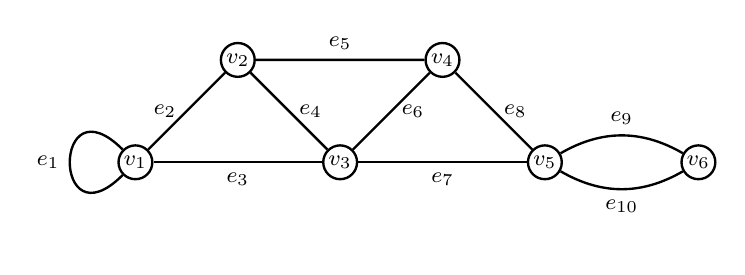
\begin{tikzpicture}[scale=1.3]
	\node[draw,inner sep=1pt,minimum size=2pt,line width=0.03cm,circle] at (0, 0)   (a) {\footnotesize$v_1$};
	\node[draw,inner sep=1pt,minimum size=2pt,line width=0.03cm,circle] at (1, 1)   (b) {\footnotesize$v_2$};
	\node[draw,inner sep=1pt,minimum size=2pt,line width=0.03cm,circle] at (2, 0)   (c) {\footnotesize$v_3$};
	\node[draw,inner sep=1pt,minimum size=2pt,line width=0.03cm,circle] at (3, 1)   (d) {\footnotesize$v_4$};
	\node[draw,inner sep=1pt,minimum size=2pt,line width=0.03cm,circle] at (4, 0)   (e) {\footnotesize$v_5$};
	\node[draw,inner sep=1pt,minimum size=2pt,line width=0.03cm,circle] at (5.5, 0)   (f) {\footnotesize$v_6$};

	\path[line width=0.03cm,out=135,in=225,looseness=10] (a) edge node[left] {\footnotesize$e_1$} (a);
	\path[line width=0.03cm] (a) edge node[left] {\footnotesize$e_2$} (b);
	\path[line width=0.03cm] (a) edge node[below] {\footnotesize$e_3$} (c);
	\path[line width=0.03cm] (b) edge node[right] {\footnotesize$e_4$} (c);
	\path[line width=0.03cm] (b) edge node[above] {\footnotesize$e_5$} (d);
	\path[line width=0.03cm] (c) edge node[right] {\footnotesize$e_6$} (d);
	\path[line width=0.03cm] (c) edge node[below] {\footnotesize$e_7$} (e);
	\path[line width=0.03cm] (d) edge node[right] {\footnotesize$e_8$} (e);
	\path[line width=0.03cm, bend left=30] (e) edge node[above] {\footnotesize$e_9$} (f);
	\path[line width=0.03cm, bend right=30] (e) edge node[below] {\footnotesize$e_{10}$} (f);
	\end{tikzpicture}
	\]

We can create a directed graph from this undirected graph by replacing each non-loop edge with a pair of edges connecting the given vertices in each direction. The resulting matrix would have the same adjacency matrix. Therefore, the matrix below have the given adjacency matrix\dots
	\[
	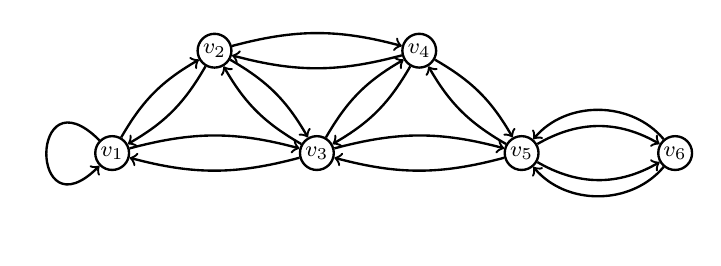
\begin{tikzpicture}[scale=1.3]
	\node[draw,inner sep=1pt,minimum size=2pt,line width=0.03cm,circle] at (0, 0)   (a) {\footnotesize$v_1$};
	\node[draw,inner sep=1pt,minimum size=2pt,line width=0.03cm,circle] at (1, 1)   (b) {\footnotesize$v_2$};
	\node[draw,inner sep=1pt,minimum size=2pt,line width=0.03cm,circle] at (2, 0)   (c) {\footnotesize$v_3$};
	\node[draw,inner sep=1pt,minimum size=2pt,line width=0.03cm,circle] at (3, 1)   (d) {\footnotesize$v_4$};
	\node[draw,inner sep=1pt,minimum size=2pt,line width=0.03cm,circle] at (4, 0)   (e) {\footnotesize$v_5$};
	\node[draw,inner sep=1pt,minimum size=2pt,line width=0.03cm,circle] at (5.5, 0)   (f) {\footnotesize$v_6$};

	\path[line width=0.03cm,out=135,in=225,looseness=10,->] (a) edge (a);
	
	\path[line width=0.03cm,bend left=15,->] (a) edge (b);
	\path[line width=0.03cm,bend left=15,->] (b) edge (a);
	
	\path[line width=0.03cm,bend left=15,->] (a) edge (c);
	\path[line width=0.03cm,bend left=15,->] (c) edge (a);
	
	\path[line width=0.03cm,bend left=15,->] (b) edge (c);
	\path[line width=0.03cm,bend left=15,->] (c) edge (b);
	
	\path[line width=0.03cm,bend left=15,->] (b) edge (d);
	\path[line width=0.03cm,bend left=15,->] (d) edge (b);
	
	\path[line width=0.03cm,bend left=15,->] (c) edge (d);
	\path[line width=0.03cm,bend left=15,->] (d) edge (c);
	
	\path[line width=0.03cm,bend left=15,->] (c) edge (e);
	\path[line width=0.03cm,bend left=15,->] (e) edge (c);
	
	\path[line width=0.03cm,bend left=15,->] (d) edge (e);
	\path[line width=0.03cm,bend left=15,->] (e) edge (d);
	
	\path[line width=0.03cm, bend left=30,->] (e) edge (f);
	\path[line width=0.03cm, bend left=50,->] (f) edge (e);
	
	\path[line width=0.03cm, bend right=30,->] (e) edge (f);
	\path[line width=0.03cm, bend right=50,->] (f) edge (e);
	\end{tikzpicture}
	\]



\newpage



% Problem 4
\problem{10} Determine which of the following graphs are isomorphic. In each case, explain the isomorphism or explains why an isomorphism cannot exist. \pspace
	\[
	\graphThree \quad \graphFour \qquad\qquad \graphFive
	\] \pspace

\sol We label these graphs from left to right as Graph~I, II, and III, respectively. Graph~I and Graph~III are isomorphic. To see this, observe that we can `pick up' the `uppermost' vertex and its edges and place it below the graph. We can then rotate the graph $180^\circ$, which results in Graph~I. We illustrate this process below. 
	\[
	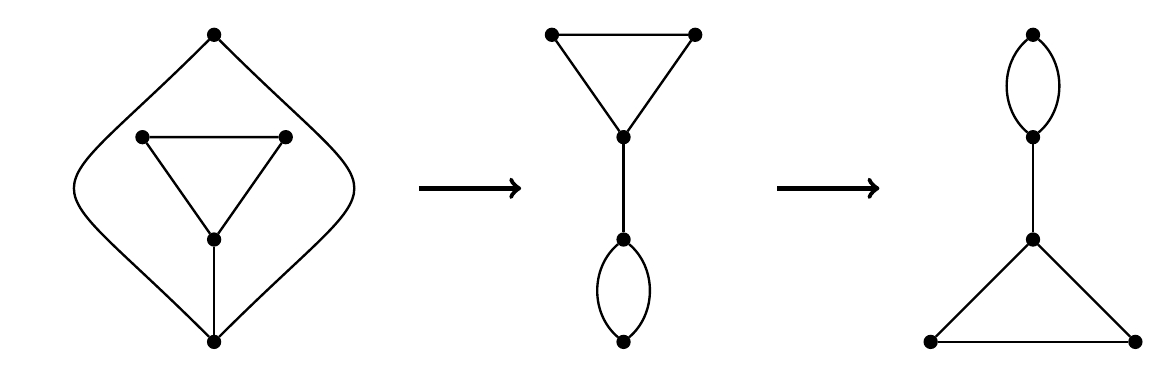
\begin{tikzpicture}[scale=1.3]
	\node[draw,inner sep=0.5pt,minimum size=1pt,line width=0.03cm,circle,fill=black] at (0, 0)   (a) {.};
	\node[draw,inner sep=0.5pt,minimum size=1pt,line width=0.03cm,circle,fill=black] at (0, 3)   (b) {.};
	\node[draw,inner sep=0.5pt,minimum size=1pt,line width=0.03cm,circle,fill=black] at (0, 1)   (c) {.};
	\node[draw,inner sep=0.5pt,minimum size=1pt,line width=0.03cm,circle,fill=black] at (-0.7, 2)   (d) {.};
	\node[draw,inner sep=0.5pt,minimum size=1pt,line width=0.03cm,circle,fill=black] at (0.7, 2)   (e) {.};
	
	\path[line width=0.03cm,bend right=45,looseness=2.2] (a) edge node[below] {} (b);
	\path[line width=0.03cm,bend left=45,looseness=2.2] (a) edge node[below] {} (b);
	\path[line width=0.03cm] (a) edge node[below] {} (c);
	\path[line width=0.03cm] (c) edge node[below] {} (d);
	\path[line width=0.03cm] (c) edge node[below] {} (e);
	\path[line width=0.03cm] (d) edge node[below] {} (e);
	
	\draw[line width=0.06cm,->] (2,1.5) -- (3,1.5);
	
	\tikzset{shift= {(4,1)}}

	\node[draw,inner sep=0.5pt,minimum size=1pt,line width=0.03cm,circle,fill=black] at (0, 0)   (a) {.};
	\node[draw,inner sep=0.5pt,minimum size=1pt,line width=0.03cm,circle,fill=black] at (0, -1)   (b) {.};
	\node[draw,inner sep=0.5pt,minimum size=1pt,line width=0.03cm,circle,fill=black] at (0, 1)   (c) {.};
	\node[draw,inner sep=0.5pt,minimum size=1pt,line width=0.03cm,circle,fill=black] at (-0.7, 2)   (d) {.};
	\node[draw,inner sep=0.5pt,minimum size=1pt,line width=0.03cm,circle,fill=black] at (0.7, 2)   (e) {.};
	
	\path[line width=0.03cm,bend right=50] (a) edge node[below] {} (b);
	\path[line width=0.03cm,bend left=50] (a) edge node[below] {} (b);
	\path[line width=0.03cm] (a) edge node[below] {} (c);
	\path[line width=0.03cm] (c) edge node[below] {} (d);
	\path[line width=0.03cm] (c) edge node[below] {} (e);
	\path[line width=0.03cm] (d) edge node[below] {} (e);
	
	\draw[line width=0.06cm,->] (1.5,0.5) -- (2.5,0.5);
	
	\tikzset{shift= {(4,-1)}}
	
	\node[draw,inner sep=0.5pt,minimum size=1pt,line width=0.03cm,circle,fill=black] at (-1, 0)   (a) {.};
	\node[draw,inner sep=0.5pt,minimum size=1pt,line width=0.03cm,circle,fill=black] at (1, 0)   (b) {.};
	\node[draw,inner sep=0.5pt,minimum size=1pt,line width=0.03cm,circle,fill=black] at (0, 1)   (c) {.};
	\node[draw,inner sep=0.5pt,minimum size=1pt,line width=0.03cm,circle,fill=black] at (0, 2)   (d) {.};
	\node[draw,inner sep=0.5pt,minimum size=1pt,line width=0.03cm,circle,fill=black] at (0, 3)   (e) {.};
	
	\path[line width=0.03cm] (a) edge node[below] {} (b);
	\path[line width=0.03cm] (a) edge node[below] {} (c);
	\path[line width=0.03cm] (b) edge node[below] {} (c);
	\path[line width=0.03cm] (c) edge node[below] {} (d);
	\path[line width=0.03cm,bend left=50] (d) edge node[below] {} (e);
	\path[line width=0.03cm,bend right=50] (d) edge node[below] {} (e);
	\end{tikzpicture}
	\]
This shows that Graph~I and Graph~III are isomorphic. \pspace

We now need to determine whether Graph~III is isomorphic to Graph~II or Graph~III. However, because being isomorphic is a transitive property, if Graph~III is isomorphic to Graph~II or Graph~III, it is isomorphic to the other. Similarly, if Graph~III is not isomorphic to Graph~II or Graph~III, it is not isomorphic to the other. Observe each graph has the same number of vertices and edges. This alone does not determine whether or not they are isomorphic. Observe the `uppermost' vertex of Graph~II had degree $1$. However, Graphs II and III do not have a vertex of degree $1$. Because isomorphisms preserve the degrees of vertices, Graph~II is neither isomorphic to Graph~I nor Graph~III. Alternatively, we can see that Graph~II has a vertex of degree $5$ while Graph~I and III do not. Alternatively, Graph I and III both have a vertex of degree $3$ while Graph~II does not. 



\newpage



% Problem 5
\problem{10} Let $G$ be an undirected graph. The \textit{degree sequence} of $G$ is a monotonic non-increasing sequence of the degrees for vertices of $G$. For instance, consider the graph from Problem~i: 
	\[
	\graphOne
	\]
This graph has degree sequence $(5, 4, 3, 2, 2, 0)$. For each of the monotonic non-increasing sequences below, determine whether they are the degree sequence for some simple graph $G$. If there is such a simple graph $G$, give an example. If no such simple graph is possible, explain why. 
	\begin{enumerate}[(a)]
	\item $(4, 3, 2, 2, 2)$
	\item $(2, 2, 2, 0)$
	\item $(5, 4, 3, 2, 1, 0)$ 
	\item $(4, 3, 3, 3, 3)$
	\item $(4, 3, 2, 1)$
	\end{enumerate} \pspace

\sol We first make a few observations about a degree sequence for a simple (undirected) graph $G$:
	\begin{itemize}
	\item {\itshape The sum of the degree sequence, $\sum_i d_i$, must be even:} We know the degree of $G$ is the sum of the degrees of its vertices. By the Handshake Theorem, we know that $\deg G$ is even. The sum of the terms of the degree sequence is the sum of the degrees of the vertices of $G$, which is $\deg G$. Therefore, this sum must be even. 

	\item {\itshape Each term of the degree sequence must be smaller than the length of the degree sequence:} Suppose a vertex $v$ had a degree $d \geq n$, where $n$ is the number of vertices. If $v$ has a loop incident to it, then $G$ is not simple, a contradiction. Otherwise, each edge of $v$ must connect $v$ to one of the other $n - 1$ vertices of $G$. Observe that $d \geq n > n - 1$. By the Pigeonhole Principle, `assigning' each of the $d $ edges incident to $v$ to a vertex of the graph, there must be a vertex with more than one edge connecting it to $v$. But then $G$ has multiple edges so that it cannot be simple, a contradiction. Therefore, $d < n$. 

	\item {\itshape If the degree sequence has length $n$, both $n - 1$ and $0$ cannot be terms in the degree sequence:} A simple graph cannot have a vertex of both degree $0$ and of degree $n - 1$. Suppose $G$ had a vertex of degree $n - 1$, say $v$. There cannot be a loop at $v$ because then $G$ would not be simple. Because $G$ is simple, there are not multiple edges between $v$ and other vertices, i.e. there is at most $1$ edge connecting $v$ to any other vertex of $G$. If $v$ was not connected to every other vertex of $G$, then there is a vertex with no edge connecting it to $v$. But then $\deg v \leq 1 + \underbrace{1 + 1 + \cdots + 1}_{n - 2 \text{ times}} < 0 + \underbrace{1 + 1 + \cdots + 1}_{n - 2 \text{ times}}= n - 2$, contradicting the fact that $\deg v= n - 1$. Therefore, $v$ is connected to every other vertex of $G$. But then $\deg v \geq 1$ for all $v \in V(G)$. But then $G$ has no vertex of degree $0$. Conversely, if there is a vertex of degree $0$, there cannot be a vertex of degree $n - 1$ because (by the previous reasoning) this vertex of degree $n - 1$ would then be connected to the degree $0$ vertex, contradicting the fact that it has degree $0$.
	
	\item {\itshape The sum of the degree sequence, $\sum_i d_i$, is at most $n(n - 1)$:} We know that $\deg G= \sum_i d_i$. Because $G$ is simple, we know that $G$ has no loops or multiple edges. We can construct a new graph, $\widetilde{G}$, as follows: $\widetilde{G}$ has the same vertex set as $G$, i.e. $V(\widetilde{G}):= V(G)$ and if $e \in E(G)$ connects vertices $v, w \in V(G)$, then $e \in E(\widetilde{G})$ connects $v, w \in V(\widetilde{G})$, i.e. $E(G) \subseteq E(\widetilde{G})$. But if $v, w \in V(G)$ are distinct vertices that do not have an edge connecting them, we add a single edge $e \in E(\widetilde{G})$ connecting $v, w$. Because $G$ had no loops and we added none through this process, $\widetilde{G}$ has no loops. Because there were no multiple edges in $G$ and we added none through this process, $\widetilde{G}$ has no multiple edges. Observe also that $\widetilde{G}$ has precisely one edge connecting any two vertices, $\widetilde{G}$ is a complete graph containing $G$ has a subgraph. Clearly, $\deg G \leq \deg \widetilde{G}$. We know that $\widetilde{G}$ has $\frac{n(n - 1)}{2}$ edges, where $n$ is the number of vertices of $G$ (which is the same number of vertices as $\widetilde{G}$). By the Handshake Theorem, $\deg \widetilde{G}= 2 |E(\widetilde{G})|= 2 \cdot \frac{n(n - 1)}{2}= n(n - 1)$. But then $\sum_i d_i= \deg G \leq \deg \widetilde{G}= n(n - 1)$.
	\end{itemize} \pspace

We will now address each of the given degree sequences. \pspace

\begin{enumerate}[(a)]
\item Observe that $\sum_i d_i= 4 + 3 + 2 + 2 + 2= 13$, which is not even. Therefore, this sequence cannot be the degree sequence of a simple undirected graph $G$. \pspace

\item There exists an undirected simple graph $G$ with degree sequence $(2, 2, 2, 0)$. For instance, the graph $G$ below has the given degree sequence. 
	\[
	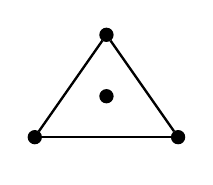
\begin{tikzpicture}[scale=1.3]
	\node[draw,inner sep=0.5pt,minimum size=1pt,line width=0.03cm,circle,fill=black] at (0, 0.4) (a) {.};
	\node[draw,inner sep=0.5pt,minimum size=1pt,line width=0.03cm,circle,fill=black] at (0, 1) (b) {.};
	\node[draw,inner sep=0.5pt,minimum size=1pt,line width=0.03cm,circle,fill=black] at (-0.7, 0) (c) {.};
	\node[draw,inner sep=0.5pt,minimum size=1pt,line width=0.03cm,circle,fill=black] at (0.7, 0) (d) {.};

	\path[line width=0.03cm] (b) edge node[below] {} (c);
	\path[line width=0.03cm] (b) edge node[below] {} (d);
	\path[line width=0.03cm] (c) edge node[below] {} (d);
	\end{tikzpicture}
	\] \pspace

\item Observe that $\sum_i d_i= 5 + 4 + 3 + 2 + 1 + 0= 15$, which is not even. Therefore, this sequence cannot be the degree sequence of a simple undirected graph $G$. Alternatively, observe the sequence $(5, 4, 3, 2, 1, 0)$ has length $n= 6$ and contains a vertex with degree $n - 1= 6 - 1= 5$ and $0$, which is impossible. \pspace

\item There exists an undirected simple graph $G$ with degree sequence $(4, 3, 3, 3, 3)$. For instance, the graph $G$ below has the given degree sequence. 
	\[
	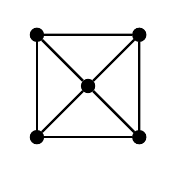
\begin{tikzpicture}[scale=1.3]
	\node[draw,inner sep=0.5pt,minimum size=1pt,line width=0.03cm,circle,fill=black] at (0, 0) (a) {.};
	\node[draw,inner sep=0.5pt,minimum size=1pt,line width=0.03cm,circle,fill=black] at (1, 0) (b) {.};
	\node[draw,inner sep=0.5pt,minimum size=1pt,line width=0.03cm,circle,fill=black] at (1, 1) (c) {.};
	\node[draw,inner sep=0.5pt,minimum size=1pt,line width=0.03cm,circle,fill=black] at (0, 1) (d) {.};
	\node[draw,inner sep=0.5pt,minimum size=1pt,line width=0.03cm,circle,fill=black] at (0.5, 0.5) (e) {.};

	\path[line width=0.03cm] (a) edge node[below] {} (b);
	\path[line width=0.03cm] (b) edge node[below] {} (c);
	\path[line width=0.03cm] (c) edge node[below] {} (d);
	\path[line width=0.03cm] (a) edge node[below] {} (d);
	
	\path[line width=0.03cm] (a) edge node[below] {} (e);
	\path[line width=0.03cm] (b) edge node[below] {} (e);
	\path[line width=0.03cm] (c) edge node[below] {} (e);
	\path[line width=0.03cm] (d) edge node[below] {} (e);
	\end{tikzpicture}
	\] \pspace

\item Observe that the sequence $(4, 3, 2, 1)$ has length $4$. Clearly, there exists a vertex with degree $4$. But then not every vertex has degree less than the length of the sequence. Therefore, there cannot be a simple undirected graph $G$ with degree sequence $(4, 3, 2, 1)$. 
\end{enumerate} \pspace

In fact, there is a general theorem that can be used to determine whether a given nonincreasing sequence of nonnegative integers is the degree sequence of a simple, undirected graph. \pspace

{\bfseries Theorem.} ({\itshape Erd\H{o}s--Gallai}) A sequence of nonincreasing, nonnegative integers $d_1 \geq d_2 \geq \cdots \geq d_n$ can be represented as the degree sequence of a finite, simple, undirected graph with $n$ vertices if and only if 
	\begin{itemize}
	\item $d_1 + d_2 + \cdots + d_n$ is even
	\item $\displaystyle \sum_{i=1}^k d_i \leq k(k - 1) + \sum_{i=k+1}^n \min(d_i, k)$ for all $1 \leq k \leq n$.
	\end{itemize}

Of course, the statement of this theorem merely states when there exists a graph $G$ with degree sequence $(d_1, d_2, \ldots, d_n)$ and not how to construct such a graph. However, there exist algorithms to construct such a graph. For instance, the Havel-Hakimi algorithm allows one to construct a graph from a degree sequence. 



\newpage



% Problem 6
\problem{10} Prove that every nontrivial simple graph has two vertices of the same degree. [Hint: Pigeonhole Principle] \pspace

\sol Let $G$ be a simple (undirected) graph with $n$ vertices, i.e. $|V(G)|= n$. If $n= 1$, then $G$ only has one vertex. Regardless of whether $G$ is simple or not, if $G$ has only one vertex, then every vertex of $G$ has the same degree---there's only one degree! Assume then that $n \geq 2$. Because $G$ is simple, it has no loops or multiple edges between vertices. We first show that if $v \in V(G)$, then $\deg v < n$. Suppose that $v \in V(G)$ with $\deg v \geq n$, i.e. $v$ is incident to $n$ or more edges. Because $G$ is simple, there cannot be a loop at $v$. But then these $\deg v \geq n$ edges incident to $v$ connect $v$ to one of the other $|V(G)| - 1= n - 1$ vertices. But then the $\deg v \geq n$ edges each connect $v$ to one of $n - 1$ possible vertices. By the Pigeonhole Principle, there must vertex $w \in V(G)$ such that there are at least two edges connecting $w$ to $v$. But then $G$ has multiple edges, contradicting the fact that $G$ is simple. \pspace

Therefore, if $v \in V(G)$, then $\deg v \in \{ 0, 1, 2, \ldots, n - 1 \}$ for all $v \in V(G)$---a total of $(n - 1) - 0 + 1= n$ possible values for $\deg v$. However, a simple graph cannot have a vertex of both degree $0$ and of degree $n - 1$. By the reasoning above, if $G$ had a vertex of degree $n - 1$, then this vertex is connected to every other vertex. But then $\deg v \geq 1$ for all $v \in V(G)$ so that there is no vertex in $G$ with degree $0$. Conversely, if there is a vertex of degree $0$, there cannot be a vertex of degree $n - 1$ because (by the reasoning above) this vertex of degree $n - 1$ would then be connected to the degree $0$ vertex, contradicting the fact that it has degree $0$. \pspace

Therefore, the possible degrees for vertices in $G$ are either $\{ 0, 1, \ldots, n - 2 \}$ or $\{ 1, 2, \ldots, n - 1 \}$. In either case, there are a total of $n - 1$ possible values for the degree of $v \in V(G)$. But then there are only $n - 1$ possible values for the degrees of the $|V(G)|= n$ vertices of $G$. By the Pigeonhole Principle, there must be two vertices that have the same degree.



\newpage



% Problem 7
\problem{10} Prove that in a tree, $T$, every pair of vertices $u$ and $v$ has a unique path connecting them. \pspace

\sol In fact, a graph $T$ is a tree if and only if there is a unique path between every distinct pair of vertices $u, v$. We prove this stronger statement. \pspace

{\itshape If $T$ is a tree, then there is a unique path between every pair of distinct vertices $u, v$:} Assume that $T$ is a tree, i.e. a connected circuit-free graph. We want to show there is a unique path for every pair of vertices $u$ and $v$. Because $T$ is connected, there exists a path between $u$ and $v$. We need only show that this path is unique. Suppose there were two distinct paths from $u$ to $v$: $u e_1 w_1 e_2 w_2 \cdots e_n w_n v$ and $u e_1' w_1' e_2' w_2' \cdots e_n' w_n' v$. 
















\newpage


{\itshape If every pair of distinct vertices has a unique edge connected them, then the graph is a tree:} Recall that a tree is a connected, circuit-free graph. Suppose a graph $G$ has a unique path between every pair of distinct vertices. Because there exists a path between every pair of vertices, $G$ is clearly connected. We need only show that $G$ is circuit free. Suppose that $G$ had a circuit. If this circuit contains only one vertex, then it must contain a loop (because the circuit contains at least one edge and only one vertex). But then there are two paths connecting $v$ to itself---the loop and the `empty path' $v$. But then $G$ does not have a unique path between every pair of vertices, a contradiction. \pspace

So suppose that $G$ contains a circuit that contains more than one vertex, say $v e_1 v_2 e_2 v_3 e_3 \cdots e_{i-1} \allowbreak v_i e_i \cdots e_{n-2} v_{n-1} e_{n-1} v$ is a circuit, where $v$ and $v_i$ are distinct vertices. Because this walk is a circuit, the edges are distinct, i.e. $e_i \neq e_j$ for $i \neq j$. Observe $v e_1 v_2 e_2 v_3 e_3 \cdots e_{i-1} v_i$ and $v e_{n-1} v_{n-1} e_{n-2} \cdots e_i v_i$ are walks from $v$ to $v_i$. These walks must be distinct because the first contains $e_1$, the second contains $e_i$, and $e_1 \neq e_i$ (because $1 \neq i$). This contradicts the fact that there is a unique path between every pair of vertices. But then $G$ cannot contain any circuits. This shows that $G$ is connected and circuit-free. Therefore, $G$ is a tree. 



\newpage



% Problem 8
\problem{10} Suppose the ground floor plan of a building is given below. Is it possible to walk through every door on the first floor exactly once, ending up in your starting room? Explain. Is it possible to visit every room exactly once, ending up in your starting room? Explain. \pspace 
	\[
	\graphSix
	\] \pspace






















\newpage



% Problem 9
\problem{10} Define the following matrices:
	\[
	A= \begin{pmatrix} 1 & 0 & -2 \\ 3 & 1 & 5 \end{pmatrix}, \quad
	B= \begin{pmatrix} 3 & 1 & -1 \\	0 & -2 & 4 \end{pmatrix}, \quad
	C= \begin{pmatrix} 1 & -1 \\ 0 & 3 \\ -2 & 1 \end{pmatrix}, \quad
	v= \begin{pmatrix} 3 \\ 0 \\-1\end{pmatrix}
	\]
For each of the following operations, either compute the given expression or explain why it is undefined. 

\begin{enumerate}[(a)]
\item $2A - B$
\item $AB$
\item $A + C$
\item $Av$
\item $AC$
\item $CA$
\end{enumerate} 

\sol One cannot only add or subtract matrices with the exact same dimension. If $A, B$ are $n \times m$ and $r \times s$ matrices, respectively, then $AB$ is defined if and only if $m= r$. If so, the product has dimension $n \times s$. 

\begin{enumerate}[(a)]
\item 
	\[
	2A - B= 2 \begin{pmatrix} 1 & 0 & -2 \\ 3 & 1 & 5 \end{pmatrix} - \begin{pmatrix} 3 & 1 & -1 \\ 0 & -2 & 4 \end{pmatrix}= \begin{pmatrix} 2 & 0 & -4 \\ 6 & 2 & 10 \end{pmatrix} - \begin{pmatrix} 3 & 1 & -1 \\ 0 & -2 & 4 \end{pmatrix}= \begin{pmatrix} -1 & -1 & -3 \\ 6 & 4 & 6 \end{pmatrix}
	\] \pspace
	
\item The product $AB$ is not defined because $A$ has $3$ columns while $B$ only has $2$ rows. \pspace

\item The sum $A + C$ is not defined because $A$ and $C$ have different dimensions. \pspace

\item 
	\[
	Av= \begin{pmatrix} 1 & 0 & -2 \\ 3 & 1 & 5 \end{pmatrix} \begin{pmatrix} 3 \\ 0 \\ -1 \end{pmatrix}= \begin{pmatrix} 1(3) + 0(0) + (-2)(-1) \\ 3(3) + 1(0) + 5(-1) \end{pmatrix}= \begin{pmatrix} 3 + 0 + 2 \\ 9 + 0 - 5 \end{pmatrix}= \begin{pmatrix} 5 \\ 4 \end{pmatrix}
	\] \pspace

\item 
	\[
	\begin{aligned}
	AC&= \begin{pmatrix} 1 & 0 & -2 \\ 3 & 1 & 5 \end{pmatrix} \begin{pmatrix} 1 & -1 \\ 0 & 3 \\ -2 & 1 \end{pmatrix} \\
	&= \begin{pmatrix} 1(1) + 0(0) + (-2)(-2) & 1(-1) + 0(3) + (-2)1 \\ 3(1) + 1(0) + 5(-2) & 3(-1) + 1(3) + 5(1) \end{pmatrix} \\
	&= \begin{pmatrix} 1 + 0 + 4 & -1 + 0 - 2 \\ 3 + 0 - 10 & -3 + 3 + 5 \end{pmatrix} \\
	&= \begin{pmatrix} 5 & -3 \\ -7 & 5 \end{pmatrix}
	\end{aligned}
	\] \pspace

\item  
	\[
	\begin{aligned}
	CA&= \begin{pmatrix} 1 & -1 \\ 0 & 3 \\ -2 & 1 \end{pmatrix} \begin{pmatrix} 1 & 0 & -2 \\ 3 & 1 & 5 \end{pmatrix} \\
	&= \begin{pmatrix} 1(1) + (-1)3 & 1(0) + (-1)1 & 1(-2) + (-1)5 \\ 0(1) + 3(3) & 0(0) + 3(1) & 0(-2) + 3(5) \\ -2(1) + 1(3) & -2(0) + 1(1) & -2(-2) + 1(5) \end{pmatrix} \\
	&= \begin{pmatrix} 1 - 3 & 0 - 1 & -2 - 5 \\ 0 + 9 & 0 + 3 & 0 + 15 \\ -2 + 3 & 0 + 1 & 4 + 5 \end{pmatrix} \\
	&= \begin{pmatrix} -2 & -1 & -7 \\ 9 & 3 & 15 \\ 1 & 1 & 9 \end{pmatrix}
	\end{aligned}
	\]
\end{enumerate}



\newpage



% Problem 10
\problem{10} Consider the graph $G$ given below: 
	\[
	\graphSeven
	\] 

\begin{enumerate}[(a)]
\item Compute the adjacency matrix, $A$.
\item Using a computer system, compute $A$, $A^2$, $A^3$, and $A^4$. 
\item Compute the number of walks from $v_1$ to $v_3$ of lengths one, two, three, and four, respectively. 
\item Compare your answers from (b) and (c). Make a conjecture on what the $a_{ij}$ entry of $A^k$ represents. 
\end{enumerate} \pspace

\sol
\begin{enumerate}[(a)]
\item The adjacency matrix is $A= (a_{ij})$, where $a_{ij}$ is the number of edges from vertex $i$ to vertex $j$. But then the adjacency matrix is\dots
	\[
	A= \begin{pmatrix}
	0 & 1 & 2 \\
	1 & 0 & 1 \\
	2 & 1 & 0
	\end{pmatrix}
	\] \pspace

\item We find that\dots
	\[
	\begin{aligned}
	A&= \begin{pmatrix} 0 & 1 & 2 \\ 1 & 0 & 1 \\ 2 & 1 & 0 \end{pmatrix} \qquad& A^3&= \begin{pmatrix} 4 & 6 & 12 \\ 6 & 4 & 6 \\ 12 & 6 & 4 \end{pmatrix} \\[0.3cm]
	A^2&= \begin{pmatrix} 5 & 2 & 1 \\ 2 & 2 & 2 \\ 1 & 2 & 5 \end{pmatrix} & A^4&= \begin{pmatrix} 30 & 16 & 14 \\ 16 & 12 & 16 \\ 14 & 17 & 30 \end{pmatrix}
	\end{aligned}
	\] \pspace

\item 














\item The number of walks of length $k > 0$ from $v_i$ to $v_j$ is the $a_{ij}$-entry of $A^k$, where $A$ is the adjacency matrix of the graph (whether directed or undirected). 
\end{enumerate}





\end{document}